\documentclass[]{article}

%opening
\title{A Mini Review on Biomarkers of Whole Grain Barley and Whole Grain Wheat Intake\footnote{This is part of Tu Hu's master thesis work, supervised by Lars Ove Dragsted and Gözde Gürdeniz}}
\author{Tu Hu}
\date{Mar, 2019}
\usepackage[backend=biber,style=nature,%sorting=ynt
]{biblatex}
\addbibresource{barley.bib}
\usepackage{graphicx}
\usepackage{tabularx}
\usepackage{makecell}
\usepackage{siunitx}
\usepackage[acronym]{glossaries}
\usepackage{footnote}
\makesavenoteenv{tabular}
\makesavenoteenv{table}
\usepackage{lscape}
\newacronym{cvd}{CVD}{cardiovascular diseases}
\newacronym{tc}{TC}{Total Cholesterol}
\newacronym{ldlc}{LDL-C}{Low Density Lipoprotein Cholesterol}
\newacronym{hdlc}{HDL-C}{High Density Lipoprotein Cholesterol}
\newacronym{tg}{TG}{Triglycerides}
\newacronym{crp}{CRP}{C-Reactive Protein}
\newacronym{wbb}{WBB}{Whole Barley Bread}
\newacronym{wwb}{WWB}{Whole Wheat Bread}
\newacronym{bfis}{BFIs}{Biomarkers of Food Intake}
\newacronym{lc-ms}{LC-MS}{Liquid Chromatography-Mass Spectrometry}
\newacronym{gc-ms}{GC-MS}{Gas Chromatography-Mass Spectrometry}
\newacronym{nmr}{NMR}{Nuclear Magnetic Resonance Spectroscopy}
\newacronym{ms/ms}{MS/MS}{Tandem Mass Spectrometry}
\newacronym{tims-pasef}{TIMS-PASEF}{Trapped Ion Mobility Spectrometry with Parallel Accumulation Serial Fragmentation}
\newacronym{hmdb}{HMDB}{Human Metabolome Database}
\newacronym{gnps}{GNPS}{Global Nature Products Social Molecular Networking}
\newacronym{aw}{AW}{After Wheat}
\newacronym{ab}{AB}{After Barley}
\newacronym{bw}{BW}{Before Wheat}
\newacronym{bb}{BB}{Before Barley}
\newacronym{pca}{PCA}{Principle Component Analysis}
\newacronym{plsda}{PLSDA}{Partial Least Squares Discriminant Analysis}
\newacronym{pqn}{PQN}{Probabilistic Quotient Normalization}
\newacronym{vip}{VIP}{variable importance in projection}

\begin{document}

\maketitle

\begin{abstract}
Due to lacking objective food exposure measurement, epidemiologic studies showed mixed results on whole grains' health beneficial effects.
Meanhile, increasing evidence showed each whole grain sub-type could benefit health differently. 
Therefore, there is a demand to discover intake biomarkers for each whole grain species.
This mini review referred the systematic biomarkers for food intake literature review guidelines and examined biomarkers for whole grain barley and whole grain wheat intake.
For whole grain barley, there is no reported intake biomarker\footnote{In my project work, I actually proposed some biomarkers}.
For whole grain wheat, the homologous ratio of alkylresorcinols C17:0/C21:0 was proposed as biomarkers to distinguish wheat and rye relative composition in the diet.

\end{abstract}

\section{Introduction}
Whole grains (WGs) and their processed food contain a lot of non-nutrient compounds in their bran parts. Besides providing carbohydrates which mostly locate in grains' endosperm, WGs may have other health beneficial effects. However, epidemiologic studies showed mixed results due to subjective self-report based food exposure measurement\cite{ISI:000447355100002}. Using \acrfull{bfis} can potentially measure food exposure in population more objectively with accuracies and details\cite{Scalbert2014}.

Alkylresorcinols (ARs) and their metabolites were widely reported and validated biomarkers for \acrshort{wgs} intake. 
In plants commonly consumed for food, \acrshort{ars} only present high amounts in rye and wheat, especially concentrated in their bran parts\cite{arreview2004}. Therefore, \acrshort{ars} have the possibility to be used as biomarkers for whole grain wheat and rye intake.

Increasing evidence showed that, different \acrshort{wg} cereal types (such as wheat, rye, oat, barley etc.) could benefit health differently. 
However, classical self-reported measurement tools (e.g. food diaries and food frequency questionnaires) used in observational studies could cause biases and confoundings to distinguish each cereal type.
Therefore, discovering \acrshort{bfis} of each whole grain type could potentially provide a tool to accurately quantify their exposures. WGs' health beneficial effects could be further elucidated. 

This mini-review aimed at systematically examining available literatures to obtain information of potential biomarkers for WG barley and wheat intake. This will prioritize further identification and validation of the thesis work.

\section{Materials and Methods}
This review referred the systematic BFIRev methodology\cite{Pratico2018}. The flowchart was included in Appendix (Fig-\ref{fig:barleybiomarkerreview})

The objective of this literature review was to identify and evaluate reported potential biomarkers for dietary assessment for whole grain wheat and whole grain barley.

Keywords as suggested in the guidelines\cite{Pratico2018} were used to search in 3 database (PubMed, Web of Science, Scopus). Keywords used for searing BFI barley in human: 
(barley) AND (biomarker* OR marker* OR metabolite* OR biokinetics OR biotransformation OR pharmacokinetics) AND (intake OR meal OR diet OR ingestion OR consumption OR eating OR food) AND 
(human* OR men OR women OR patient* OR volunteer* OR participant*) AND 
(trail* or experiment OR study) AND (urine OR plasma OR blood OR serum OR excretion OR hair OR toenail OR faeces OR faecal water). The first element was changed to wheat for wheat intake biomarker searching. 

Due to limited amount of searching results, barley searching scope was expanded to animal studies. Therefore, the keyword (animal* OR goat OR sheep OR cow OR mice OR mouse* OR animal model* OR dog*) was used to replace the previous 'human*' subjects. In addition, 'feed' was added to 'food' entry.

Other database including HMDB\cite{hmdb}, FoodDB\cite{foodb}, PhenolExplorer\cite{phenolexplorer}, Dictionary of Food Compound\cite{dictionary} were also used to explore compounds present only in \acrshort{wg} barley and wheat. 

In order to verify the uniqueness of compound, the same keywords combinations were used but with compound instead of 'wheat' and 'barley'.

\section{Results}
\subsection{WG barley}
The literature search got 129 records after removing duplicates from merged 3 database search results. However, within them, none of the studies directly investigated WG barley intake biomarkers. This could be explained by limited consumption of barley in population. Although barley is the 4th most produced cereal grains worldwidely. Most of them is used for brewing or feed. Approximately only 4\% is directly consumed\cite{Baik2008}.

When the scope expanded to animal studies, the search results still did not show any direct research about BFIs. Most of animal studies were interested in how barley feed can benefit the growth of animals or quality improvement of animal-source products\cite{ISI:000272990200002,Foster2003}.

A 2-month intervention study\cite{DeAngelis2015} incorporated 75\% refined drum wheat and 25\% WG barley. The fecal samples showed significant change in microbiota and metabolome after intervention\cite{DeAngelis2015}. However, no specific metabolite can indicate WG barley intake.

ARs and their metabolites may not indicate WG barley intake. Several observation studies\cite{ISI:000309032000011,ISI:000259554500019} investigated correlation between ARs metabolites and whole grain intake. Although these studies tried to cover more whole grain species, for example, one study\cite{ISI:000259554500019} listed 7 types of commonly consumed WGs in American populations in the \acrfull{ffq}\footnote{Dark breads, High-fiber or bran cereals, Cooked cereals and grits, Regular granola, Granola bars and cereal bars, Plain popcorn (no butter) or low-fat microwave popcorn, Buttered or gular microwave popcorn}, barley was not solely listed. Therefore, although ARs and their metabolites got good correlation with these 'Whole-grain intake'. Readers should be cautious to apply these markers to \acrshort{wg} barley intake. 
In addition, ARs concentration in cereal barley is much lower compared with \acrshort{wg} wheat and rye, with similar concentration with refined wheat and rye flours (Table-\ref{table:ars_in_plant}). 

\begin{table}[h!]
		\footnotesize
\centering
\begin{tabular}{|c|c|c|c|c|c|}
	\hline 
	Cereal & \makecell{Conc. range \\in cereal}& \makecell{Conc. average \\or range \\in WG flour }& \makecell{Conc. average \\in refined \\flour} & \makecell{Main\\homologues} & \makecell{C17:C21\\ homologues\\ratio} \\ 
	\hline 
	Rye&360-3200& 972 &90&C17, C19, C21& 0.8-0.9 \\ 
	\hline 
	Wheat&761-8390& 490-710 & 36& C19, C21& 0.07-0.1 \\ 
	\hline 
	Barley& 55.8-98.2&NA & NA& C19, C21, C25&NA  \\ 
	\hline 
\end{tabular} 
	\caption{Prensence of ARs in Cereal Grains, adapted from \cite{doi:10.1021/jf0340456,ANDERSSON2010794,BORDIGA201638}(unit: \SI{}{\micro\gram}/g dm), conc. varies due to different species and milling methods.}
	\label{table:ars_in_plant}
\end{table}

Most search results focused on barley's \textit{effect biomarkers} as defined by Dragsted\cite{Dragsted2017} and Gao\cite{Gao2017}, such as bowel health indicators\cite{Bird2008}, postprandial glucose and insulin response\cite{Ames2015}, lipid profiles and \acrfull{cvd} markers\cite{Marungruang2018}, etc. However, in these intervention studies, compliance monitoring lacked objective markers.

Further search results in food chemistry, cereal science and plant science showed some compounds exclusively present in barley. These could give hints for further identification. The results were summarized in Table-\ref{table:candidate_biomarker_barley}.

\begin{table}[h!]
	\centering
	\small
\scalebox{0.78}{
\begin{tabular}{|c|c|c|c|c|c|}
	\hline 
	No & \makecell{Candidate\\biomarker}& Formula & \makecell{Chemical\\group} &Presence in Food & Reference\\ 
	\hline 
	1&Hordenine& C\textsubscript{10}H\textsubscript{15}NO &alkaloid&\makecell{germinating barley,\\ beer and other plants}&\cite{Gurdeniz2016}\\ 
	\hline
	4&Hordatine A&C\textsubscript{28}H\textsubscript{38}N\textsubscript{8}O\textsubscript{5}&alkaloid&\makecell{only reported\\in barley}&\makecell{FoodDB\\(002330)}\\ 
	\hline 
	4&Hordatine B&C\textsubscript{29}H\textsubscript{40}N\textsubscript{8}O\textsubscript{5}&alkaloid&\makecell{only reported\\in barley}&\makecell{FoodDB\\(002328)}\\ 
	\hline 
	2&\makecell{Distichonic\\acid A}&C\textsubscript{10}H\textsubscript{18}N\textsubscript{2}O\textsubscript{8}&\makecell{gamma amino acids\\ and derivatives}&\makecell{only reported\\in barley}&\makecell{FoodDB\\(18164)}\\
	\hline 
	3&\makecell{Distichonic\\acid B}&C\textsubscript{10}H\textsubscript{18}N\textsubscript{2}O\textsubscript{8}&\makecell{gamma amino acids\\ and derivatives}&\makecell{only reported\\in barley}&\makecell{FoodDB\\(018165)}\\ 
	\hline 
	
	5&\makecell{14,16-Nona\\cosanedione}&C\textsubscript{29}H\textsubscript{56}O\textsubscript{2}&ketone&\makecell{only reported\\in barley}&\makecell{FoodDB\\(013891)}\\ 
	\hline 
	6&N-Norgramine&C\textsubscript{10}H\textsubscript{12}N\textsubscript{2}&indole&\makecell{only reported\\in barley}&\makecell{FoodDB\\(017815)}\\ 
	\hline 
\end{tabular} }
\caption{Candidate Biomarkers for WG barley intake}
\label{table:candidate_biomarker_barley}
\end{table}
To conclude, barley, especially \acrshort{wg} barley attracted a lot of interest due to its health beneficial effects for chronic disease. However, due to barley's limited consumption in the population, currently there is no reported biomarkers can indicate its intake. A lot of sparse information was reported from cereal and food chemistry could give hints for identification and validations of \acrshort{wg} barley's intake biomarkers.

\subsection{WG wheat}
\subsubsection{Overview}
The literature search got 312 results after removing duplicates from merged results. Some articles were found from the references of searched results. 
\textbf{One intervention study and one observation study} %% May be changed afterwards
were included in the table. 

%%% EXPLAIN WHY SO FEW RESULTS WERE INCLUDED
%%% I think this overview needs to be improved
Surprisingly few studies of whole grain wheat intake biomarkers were reported because whole grains seem to be the hotspot and mostly researched area of \acrshort{bfis}.
%% NOT QUITE SURE IT'S CORRECT OR NOT. 
In fact, within searched results, most intervention studies used \acrshort{wg} diet containing several types of cereals as a comparison with refined diet, most commonly using \acrshort{wg} rye and wheat and reporting ARs as intake biomarkers for \acrshort{wg} rye and wheat. Very few intervention studies investigated biomarkers for different whole grains' intake. 

%% My research question is to find marker specific for WG wheat.

%% OBSERVATIONAL STUDY
FOR EXAMPLE, IN THIS STUDY\cite{ISI:000348343300015}, SUBJECTS WERE CLASSIFIED AS CONSUMER OF 'NONE-BREAD', 'WHITE BREAD' AND 'WHOLE GRAIN BREAD'. HOWEVER, WE DO NOT KNOW, WHICH TYPE OF CEREAL GRAINS ARE THE BREAD MADE OF. THESE BIOMARKERS ARE LESS USEFUL FOR OUR IDENTIFICATIONS.

In observational studies, estimations of food exposure are based on self-report.

Therefore, it is difficult to assign the biomarker to the specific food.

Food frequency questionnaire causes high deviations distingushing each sub-type cereal by its nature. Because participants had difficulty recalling and distinguishing the different cereal species.

Those non-specific markers were listed in appendix. 
These ambiguous studies were excluded.
However, still surprising to us, few researches were studied to distinguish wheat from other cereal grains.

However, ar can only indicate whole grain wheat and rye intake but not other whole grain cereals. assuming someone eats a lot of whole grain oat or 


\subsubsection{Alkylresorcinols (ARs) and AR metabolites}
\acrfull{ars} have the potential to indicate WG wheat and rye intake. 
Because within commonly consumed plant-based food, alkylresorcinols present high concentration exclusively in bran part of wheat and rye. 

Total alkylresorcinols and their metabolites (3,5-DHPPTA, 3,5-DHPPA, 3,5-DHBA and 3,5-DHBA glycine) were not specific to WG wheat but got good correlations with WG wheat intake in rye rarely consumed countries, such as UK and USA. In these countries, WG wheat is the only alkylresorcinol source.

%%%super important
\acrshort{ars} are absorbed by humans and can be detected in blood plasma, erythrocytes, adipose tissue\cite{ISI:000451002000016}, and in the form of polar metab- olites in urine

%%%detection method
AR metabolites: urine/plasma: HPLC-COULOMETRIC ELECTRODE ARRAY DETECTOR

%%%METABOLITES
longer apparent half-lives

\begin{figure}[h!]
	\centering
	\includegraphics[width=0.5\linewidth]{picture/ars_sang_pathway}
	\caption{Structure of \acrshort{ars} and suggested metabolic pathway, adapted from \cite{ISI:000447355100002}}
	\label{fig:structure_ars}
\end{figure}

\subsubsection{AR homologous ratio C17:0/C21:0}
In wheat and rye both consumed countries, total ARs and ARs metabolites indicate WG wheat and rye intake, while AR homologous ratio C17:0/C21:0 can indicate relative compositions of WG wheat and rye in the diet.

AR homologous ratio C17:0/C21:0 was first reported by cereal scientists in 2004 to distinguish \acrshort{wg} rye and wheat cereal \cite{Chen2004}. In grains, rye has homologous C17:0/C21:0 ratio close to 1.0, while wheat around 0.1, durum wheat around 0.01.

Further this marker was proposed by nutritionists to distinguish \acrshort{wg} rye and wheat intake. In 2005, Linko\cite{ISI:000376712600013} first investigated this biomarker in human plasma to measure food exposure. The intervention study showed the potential of this marker AR C17:0/C21:0 to distinguish \acrshort{wg} wheat and rye in diet in healthy postmenopausal women. 
For rye-dominated diet, the ratio was 0.84 and for WG wheat-dominated diet, the ratio was around 0.53. 
Further in 2007, Linko-Parvinen validated this marker in healthy adults by an intervention study \cite{10.1093/jn/137.5.1137}.
In plasma, the value was 0.1 after WG wheat intake, 0.6 after WG rye intake. In erythrocytes, the value was 0.06, 0.33 respectively after WG wheat and rye intake. This study also implied ARs could be transported in human plasma lipoproteins.

However, the AR homologues ratio C17:0/C21:0 was not significantly different between \acrshort{wg} diet and refined cereal diet as reported by Landsberg\cite{ISI:000255012000007}. But WG diet and refined diet can be distinguished by total ARs concentration in plasma.

An observational study further validated this marker.
In 2014, EPIC\footnote{European Prospective Investigation into Cancer and Nutrition} cohort study investigated plasma ARs and the C17:0/C21:0 ratio of subjects from 10 European countries. 
The result showed that Greek, Italian, Dutch and UK participants of whom the diet was dominated by wheat, had low C17:0/C21:0 ratio in plasma. Whereas Danish, German and Swedish subjects had high C17:0/C21:0 ratio. French and Norwegian subjects had intermediate ratio. This marker seems reversely correlated with WG wheat consumption in the population.

%\acrshort{ars} (Figure\ref{fig:structure_ars}) and their metabolites  were widely reported, validated and applied biomarkers for WG wheat and rye intake. 
%Total \acrshort{ars} were used as biomarkers for overall \acrshort{wgs} wheat and rye exposure. In order to distinguish \acrshort{wg} wheat and rye. The ratio of C17:0/C21:0 was used. \acrshort{ars}, depending on different milling methods and grain species, varies the concentration and homologues compositions (Table-\ref{table:ars_in_plant}). . The ratio was further proposed as an marker to indicate which cereal dominates in the diet: if the ratio is close to 1.0, rye dominated; close to 0.1, wheat dominates\cite{ISI:000376712600013,Landberg2009}.



%%%%%%%%%%% WHEAT INTERVENTION
\begin{table}[h!]
	\scalebox{0.83}{
\begin{tabular}{|c|c|c|c|c|c|c|c|}
	\hline 
	\makecell{Dietary\\factor} & \makecell{No.\\subjects} & \makecell{Study\\design}  & \makecell{Sample\\type}  & \makecell{Analytical\\method}& \makecell{Candidate\\biomarker(s)} & Reference \\ 
	\hline 
	
	\makecell{WG wheat\\WG rye} & 39 & \makecell{intervention,\\ cross-over,\\ randomized} & plasma & GC-MS & \makecell{ratio of AR\\C17:0/C21:0} & \cite{ISI:000376712600013} \\ 
	\hline 
	
	%\makecell{\makecell{Healthy\\ new \\nordic\\diet\footnote{containing more rye than control group}}} & 166 & \makecell{intervention,\\ parallel,\\ randomized,\\ multi-center\\ (18/24 weeks)} & plasma & GC-MS & \makecell{ratio of AR\\C17:0/C21:0} & \cite{ISI:000333777700008} \\ 
	%\hline 
	

\end{tabular} }
\caption{Biomarkers of Wheat Intake Reported in Intervention study}
\label{table:wheat_intervention}
\end{table}

%In \acrfull{wg} source dominated by wheat, total ARs got good correlation with wheat intake. e.g. UK and America. 

%Meanwhile, ARs metabolites could also be a potential marker, but may not be a good marker in mixed-ARs source countries since ARs metabolites were not specific to WG wheat. 
%ARs from WG rye could also be metabolized to same products causing confounding.
%%%%%%%%%% WHEAT OBS
\begin{table}[h!]
	\scalebox{0.83}{
		\begin{tabular}{|c|c|c|c|c|c|c|}
			%header
			\hline 
			\makecell{Type of\\ WG} & \makecell{No.\\subjects} & \makecell{Sample\\type}  & \makecell{Analytical\\method} & \makecell{Candidate\\biomarker(s)} & \makecell{Associated\\with} & Reference \\ 
			\hline
			%%EU cohort
			WGs\footnote{This cohort studies investigated WGs conc. in different EU countries' population.} & 2845 & \makecell{\makecell{fasting and \\non-fasting\\plasma}}  & GC-MS & AR C17:0/C21:0 & FFQ & \cite{ISI:000334172400017} \\ 
			\hline	
			
	\end{tabular}}
	\caption{Biomarkers of Wheat Intake Reported in Observation study}
	\label{table:wheat_observation}
\end{table}
%In this study\cite{ISI:000298402100026}, total ARs, rather than the ratio (C17:0/C21:0), were reported as \acrshort{wg} wheat intake biomarkers.
%This intervention was conducted in UK. In British population, the major whole grain source is wheat. Rye was rarely consumed. Therefore, plasma ARs got a good correlation with \acrfull{wg} wheat intake.

\subsubsection{Applications in Type II diabetes research}
Combining plasma total ARs concentration and the ratio (C17:0/C21:0) can subjectively estimate \acrshort{wg} wheat and rye intake and approximate relative compositions in the diet. This will provide more detailed information regrading intake amount of specific cereal species.

For example, an observation study showed, in Chinese population AR metabolite DHPPA was correlated with lower odds of type II diabetes and impaired glucose regulation\cite{ISI:000430455900021}. However, DHPPA as AR metabolite can come from either whole grain wheat or rye.

Other two researches can better show that, actually \acrshort{wg} rye could be more favorable for type II diabetes.  An observational study showed in a population with metabolic syndrome, plasma AR C17:0/C21:0 was associated with increased insulin sensitivity\cite{ISI:000333777700008}. Further, it was observed that in healthy Scandinavian populations, plasma total ARs concentration was not correlated with type II diabetes risk. However higher C17:0/C21:0 ratio (implicating more rye intake) was associated with increased insulin sensitivity\cite{ISI:000378977200013}. These results imply that, a whole grain diet dominated by rye could be favourable for type II diabetes prevention. 

In EPIC cohort study, an interesting phenomena could also imply XXX. Rye has higher constitutions in Danish populations's WG source (70\%) than Swedish (55\%) on average. Regarding C17:0/C21:0 ratio, Danish participants in EPIC cohort showed lower value (0.37) than Swedish participants (0.43). 
However, Swedish participants were healthy adults, while participants from Denmark in EPIC study were obese or over-weights subjects. Those participants may have different dietary habits and consume less rye than average Danes. This may imply rye could also be favorable in weight control.

All these observation studies indicate that, application of biomarkers for sub-type ceral may be more powerful to rather than a overall WG intake.

\subsubsection{Other potential markers}
Searching results also showed some \textit{Food compound intake biomarkers (FCIBs)} research as defined by Gao\cite{Gao2017} such as phenolic compounds\cite{ISI:000389134200003}, benzoxazinoids (BXOs)\cite{ISI:000394168100034,ISI:000348343300015}, phytoestrogen\cite{ISI:000384082300001}, phytosterol and lignan\cite{ISI:000387249200001}, MICROBIOAL DERIVITIVES\cite{ISI:000348343300015}. These compounds also present in other food,  not specific for \acrshort{wg} wheat. These results were summarized in Appendix.

In this article{ISI:000387249200001}, author performed an intervention study using refined wheat bread as control group, authors proposed a panel of metabolites consisting 7 AR metabolites, 5 BXO metabolites and 5 phenolic acid derivatives can be used to objectively monitor WG wheat intake. However, this conclusion needs to be further identified in other intervention and observation studies.

Their concentrations varied in different cereal grains. Therefore, a combination of their metabolites could potentially indicate intake of different cereals.


%% conclusion
to conclude, AR 17/21 seems promising 

\section{Conclusions}
%\acrshort{wg} barley attracted a lot of interest due to its health beneficial effects for preventing chronic disease. However, 
None biomarker has been reported for \acrshort{wg} barley intake both from human and animal studies.

Total \acrshort{ars} from plasma can indicate WG rye and wheat intake.
The homologues ratio of \acrshort{ars} C17:0/C21:0 can indicate relative composition of WG rye and wheat. Combing these two markers can objectively indicate \acrshort{wg} wheat intake. This marker has been implemented in several studies and proven its usefulness.
\section{Discussions}
In order to clarify each sub-type of cereal's health beneficial effects, it is important to accurately quantify exposure amount of each sub-type. BFIs showed their strengths and potentials in studying WGs. 


it is essential to discover intake biomarker for each sub-type cereal grain.
Currently, most studies showed interest in WG effect biomarkers.

As discussed in \cite{ISI:000447355100002}, one of the challenges in BFIs discovery of WG is that the chemical compositions of most of WGs were not systematically 

due to limited systematic research on phytochemicals 



\section{Appendix}
\begin{table}[h!]
	\centering
	\small
	\scalebox{0.78}{
		\begin{tabular}{|c|c|c|c|c|c|}
			\hline 
			No & \makecell{Candidate\\biomarker}& Formula & \makecell{Chemical\\group} &Presence in Food & Reference\\ 
			\hline 
			1&Hordenine& C\textsubscript{10}H\textsubscript{15}NO &alkaloid&\makecell{germinating barley,\\ beer and other plants}&\cite{Gurdeniz2016}\\ 
			\hline
			4&Hordatine A&C\textsubscript{28}H\textsubscript{38}N\textsubscript{8}O\textsubscript{5}&alkaloid&\makecell{only reported\\in barley}&\makecell{FoodDB\\(002330)}\\ 
			\hline 
			4&Hordatine B&C\textsubscript{29}H\textsubscript{40}N\textsubscript{8}O\textsubscript{5}&alkaloid&\makecell{only reported\\in barley}&\makecell{FoodDB\\(002328)}\\ 
			\hline 
			2&\makecell{Distichonic\\acid A}&C\textsubscript{10}H\textsubscript{18}N\textsubscript{2}O\textsubscript{8}&\makecell{gamma amino acids\\ and derivatives}&\makecell{only reported\\in barley}&\makecell{FoodDB\\(18164)}\\
			\hline 
			3&\makecell{Distichonic\\acid B}&C\textsubscript{10}H\textsubscript{18}N\textsubscript{2}O\textsubscript{8}&\makecell{gamma amino acids\\ and derivatives}&\makecell{only reported\\in barley}&\makecell{FoodDB\\(018165)}\\ 
			\hline 
			
			5&\makecell{14,16-Nona\\cosanedione}&C\textsubscript{29}H\textsubscript{56}O\textsubscript{2}&ketone&\makecell{only reported\\in barley}&\makecell{FoodDB\\(013891)}\\ 
			\hline 
			6&N-Norgramine&C\textsubscript{10}H\textsubscript{12}N\textsubscript{2}&indole&\makecell{only reported\\in barley}&\makecell{FoodDB\\(017815)}\\ 
			\hline 
	\end{tabular} }
	\caption{Potential Biomarkers for WG Barley Intake}
	\label{table:candidate_biomarker_barley}
\end{table}

\begin{figure}[h!]
	\centering
	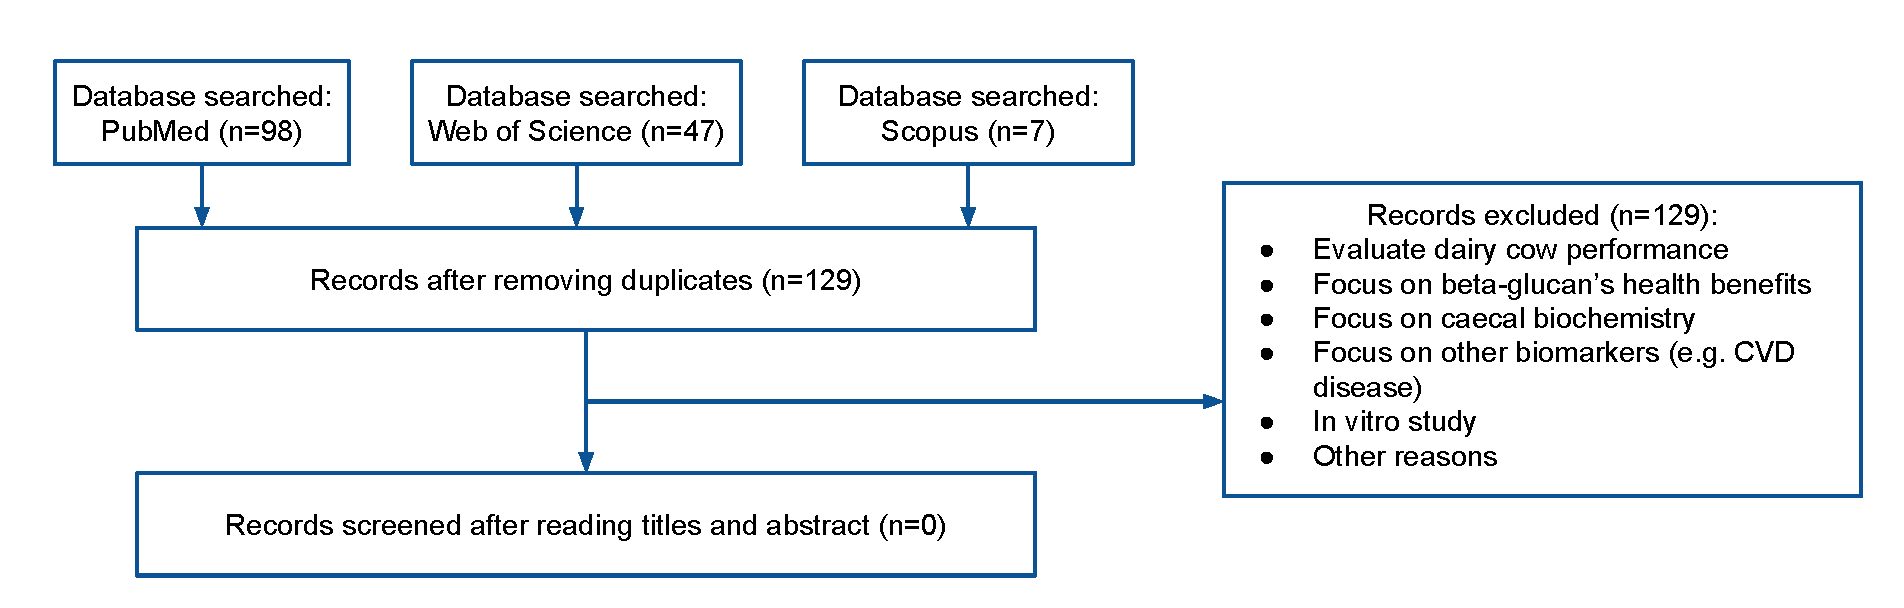
\includegraphics[width=\linewidth]{picture/barley_biomarker_review}
	\caption{Flow Chart of Literature Searching and Screening for Articles of WG Barley Intake Biomarkers}
	\label{fig:barleybiomarkerreview}
\end{figure}

\begin{figure}[h!]
	\centering
	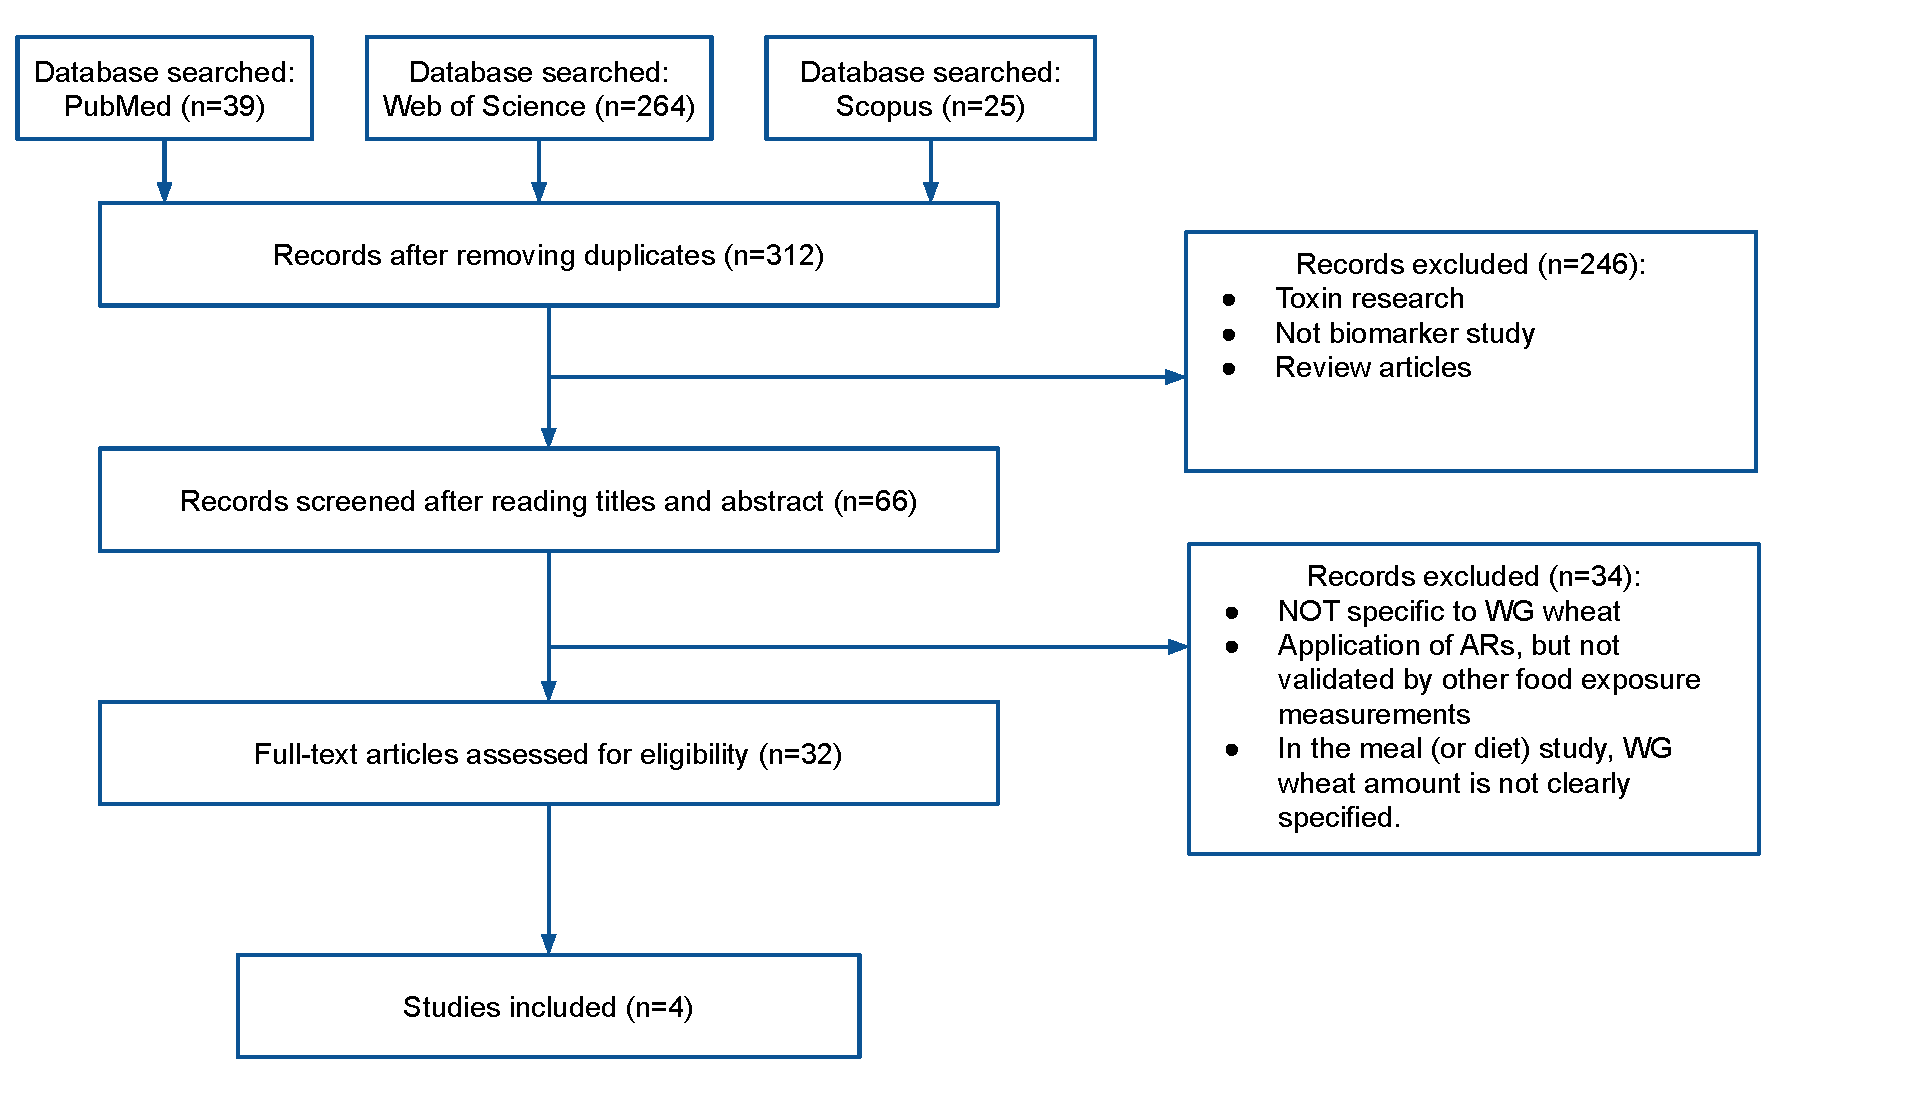
\includegraphics[width=\linewidth]{picture/wheat_biomarker_review}
	\caption{Flow Chart of Literature Searching and Screening for Articles of WG Wheat Intake Biomarkers}
	\label{fig:wheatbiomarkerreview}
\end{figure}

%%%%
{\centering
%\begin{landscape}
	\begin{table}[h!]
		\scalebox{0.7}{
			\begin{tabular}{|c|c|c|c|c|c|c|}
				%header
				\hline 
				\makecell{Dietary\\factor} &  \makecell{No.\\subjects} &\makecell{Study\\design} & \makecell{Sample\\type}  & \makecell{Analytical\\method} & \makecell{Candidate\\biomarker(s)} & Reference \\ 
				\hline
				%1st entry - betaine
				\makecell{Wheat bran,\\Wheat aleurone} & 14+13 & \makecell{randomized,\\ cross-over,\\ intervention} & \makecell{plasma}  & \makecell{LC-MS/MS\\ (Microbiology assay\\for folate)} & \makecell{betaine\\choline\\folate\\dimethylglycine (DMG)} & \cite{ISI:000350230300006} \\ 
				\hline
				
				%2nd entry - PREDIMED
				\makecell{None-bread,\\White bread,\\WG bread} & 155 & observation\footnote{dietary exposure measured from FFQ} & \makecell{\makecell{urine}}  & HPLC-qTOF-MS & \makecell{Benzoxazinoid-related metabolites\\(HHPAA, HBOA glycoside)\\ ARs-related metabolites\\ (DHPPA glucuronide, DHPPTA sulphate\\microbial-derived metabolites} & \cite{ISI:000348343300015} \\ 
				\hline
				
				%3rd entry
				%WGs\footnote{This study was conducted in US. WG wheat is the major WG source in US populations. However, these two metabolites were not specific to WG wheat. Because other cereals containing ARs could also be metabolized to these metabolites.} & 104 & observation (FFQ)& \makecell{spot\\urine}  & GC-MS & \makecell{ARs metabolites\\(DHBA, DHPPA)} & \cite{ISI:000303089700010} \\ 
				%\hline		
				%\hline 
				
				%4th entry
				%\makecell{WGs\footnote{This study was conducted in UK. WG wheat is the main WG source in British population. Considering this, although several types of WGs were used (WG wheat, corn, oats, barley and rice), WG wheat made up around 65\% of the intervention}} & 266 & \makecell{randomized,\\ parallel-group,\\ intervention} & plasma & GC-MS & Total ARs & \cite{ISI:000298402100026} \\ 
				%\hline 
				\end{tabular}}
		\caption{Reported markers distinguishing WG wheat intake, but NOT specific}
		\label{table:wheat_notspecific}
	\end{table}
}
%\end{landscape}}


\clearpage
\printbibliography[
heading=bibintoc,
title={References}
]
\end{document}
